%!TEX root = ../main.tex

\newpage
\section*{Tables and Figures}

% Tables

  \begin{table}[h]
    \centering
    \small
    \begin{tabular}{|c|c|c|c|}
      \hline
      \textbf{Workflow step} & \textbf{Module/Condition} & \textbf{Tool/Parameter} & \textbf{References/Value} \\
      \hline
      \multirow{7}{*}{Denoising and Clustering} & \multirow{5}{*}{Denoise and Cluster} & Closed reference & \cite{rognesVSEARCHVersatileOpen2016,bolyenReproducibleInteractiveScalable2019} \\
                                                &  & Open reference & \cite{rognesVSEARCHVersatileOpen2016,bolyenReproducibleInteractiveScalable2019} \\
                                                &  & De novo & \cite{rognesVSEARCHVersatileOpen2016,bolyenReproducibleInteractiveScalable2019} \\
                                                &  & Dada2 & \cite{Callahan2016} \\
                                                &  & Deblur & \cite{Amir2017,bolyenReproducibleInteractiveScalable2019} \\
                                                \cline{2-4}
                                                & \multirow{2}{*}{Chimera checking} & Uchime-denovo & \cite{rognesVSEARCHVersatileOpen2016,bolyenReproducibleInteractiveScalable2019} \\
                                                & & Remove bimera & \cite{Callahan2016} \\
                                                \hline
      \multirow{5}{*}{Taxonomy assignment} &  \multirow{2}{*}{Query tool} & Blast & \cite{camachoBLASTArchitectureApplications2009,bokulichOptimizingTaxonomicClassification2018} \\
                                           &  & Naive bayes classifier & \cite{bokulichOptimizingTaxonomicClassification2018} \\
                                           \cline{2-4}
                                           & \multirow{3}{*}{Database} & Greengenes & \cite{DeSantis2006} \\
                                           & & SILVA & \cite{Quast2012} \\
                                           & & NCBI RefSeq & \cite{Sayers2009} \\
      \hline
      \multirow{6}{*}{OTU processing} & \multirow{3}{*}{Filter(off)} & Prevalence threshold      & 2 / n\_samples \\
                                      & & Abundance threshold       & 0.001          \\
                                      & & Observation sum threshold & 10             \\ \cline{2-4}
                                      & \multirow{3}{*}{Filter(on)}  & Prevalence threshold      & 0.05           \\
                                      & & Abundance threshold       & 0.01           \\
                                      & & Observation sum threshold & 100            \\
      \hline
      \multirow{12}{*}{Network Inference} & \multirow{2}{*}{Bootstrapping}& \texttt{fastspar\_bootstraps} v1.0 & \cite{Watts2018} \\
                                          & & \texttt{fastspar\_pvalues} v1.0 & \cite{Watts2018} \\
                                          \cline{2-4}
                                          & \multirow{6}{*}{Direct association} & \ac{spieceasi} v1.1.2 & \cite{Kurtz2015} \\
                                          & & FlashWeave.jl v0.18.1 & \cite{tackmannRapidInferenceDirect2019} \\
                                          & & \ac{cozine} v1.0 & \cite{haCompositionalZeroinflatedNetwork2020a} \\
                                          & & \ac{harmonies} v1.0 & \cite{jiangHARMONIESHybridApproach2020} \\
                                          & & \ac{spring} v1.0.4 & \cite{yoonMicrobialNetworksSPRING2019} \\
                                          & & \ac{mldm} v1.1 & \cite{Yang2017} \\
                                          \cline{2-4}
                                          & \multirow{2}{*}{Correlation-based} & FastSpar (\ac{sparcc}) v1.0 & \cite{Watts2018} \\
                                          & & Pearson & - \\
                                          & & Spearman & - \\
                                          & & propr v2.1.2 & \cite{quinnProprRpackageIdentifying2017} \\
      \hline
    \end{tabular}
    \caption{Tools used in the \ac{micone} pipeline}
    \label{tab:micone_tools}
  \end{table}

  \begin{table}[h]
    \centering
    \small
    \begin{tabular}{|c|c|c|}
      \hline
      \textbf{Workflow step} & \textbf{Default tool} \\
      \hline
      Denoising and Clustering & Dada2 and remove bimera \\
      Taxonomy Assignment & \ac{gg} with NaiveBayes classifier \\
      OTU Processing & Thresholds on prevalence and abundance \\
      Network Inference & scaled-sum consensus method \\
      \hline
    \end{tabular}
    \caption{Default tools and parameters of the \ac{micone} pipeline}
    \label{tab:default_options}
  \end{table}


% Figures
  \FloatBarrier
  \newpage

  \begin{figure}[h]
    \centering
    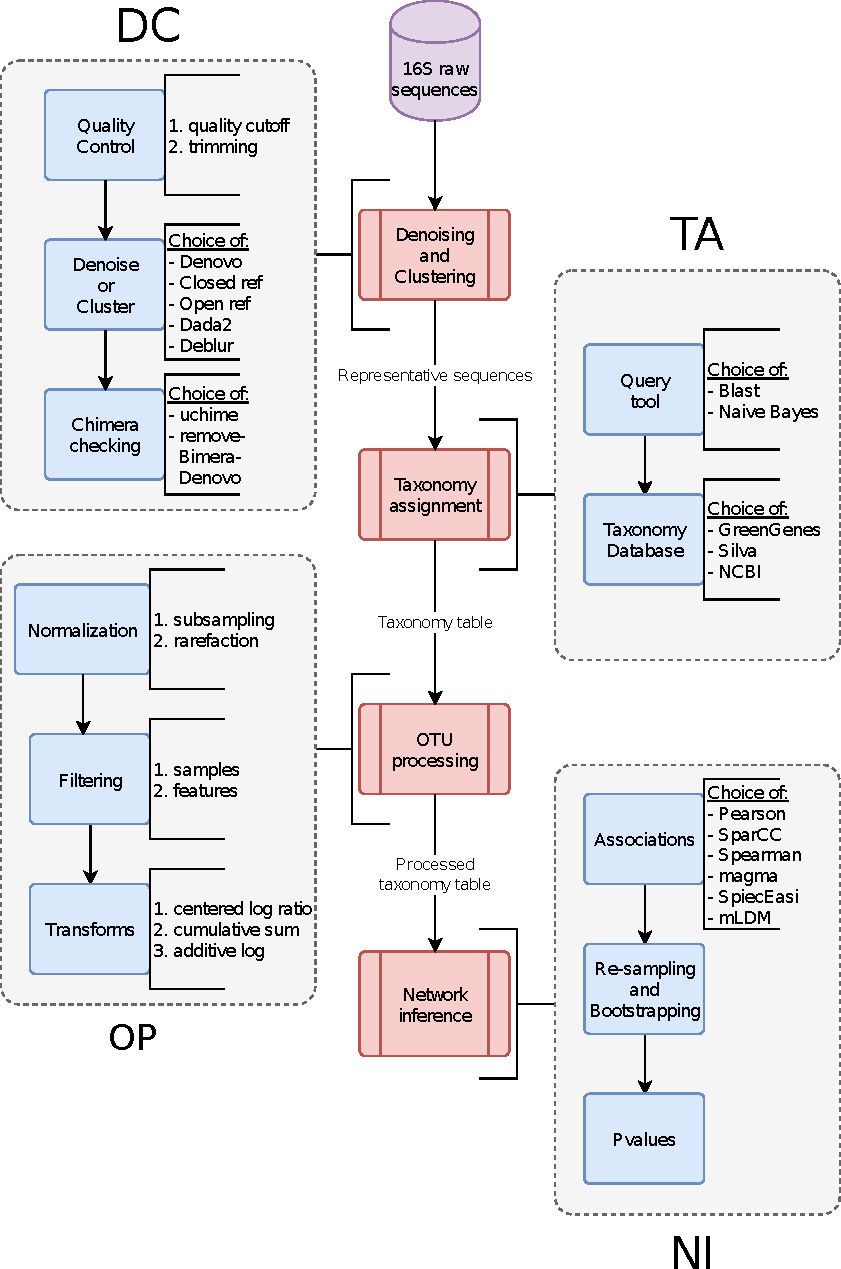
\includegraphics[width=0.74\linewidth]{figure1.pdf}
  \end{figure}
  \begin{figure}[ht!]
    \centering
    \caption{
      \textbf{The workflow of the \ac{micone} pipeline}.
      The steps can be grouped into five major groups: \textbf{(SP)} \textbf{S}equence \textbf{P}rocessig, \textbf{(DC)} \textbf{D}enoising and \textbf{C}lustering, \textbf{(TA)} \textbf{T}axonomy \textbf{A}ssignment, \textbf{(OP)} \textbf{O}TU or ESV \textbf{P}rocessing, and \textbf{(NI)} \textbf{N}etwork \textbf{I}nference.
      Each step incorporates several processes, each of which in turn have several alternate algorithms for the same task (indicated by the text to the right of the blue boxes).
      The text along the arrows describes the data that is being passed from one step to another.
      The final output of the pipeline are consensus networks generated from the co-occurrence networks.
      For details on each process and data types, see Methods.
    }
    \label{fig:figure1}
  \end{figure}

  \FloatBarrier
  \newpage

  \begin{figure}
    \centering
    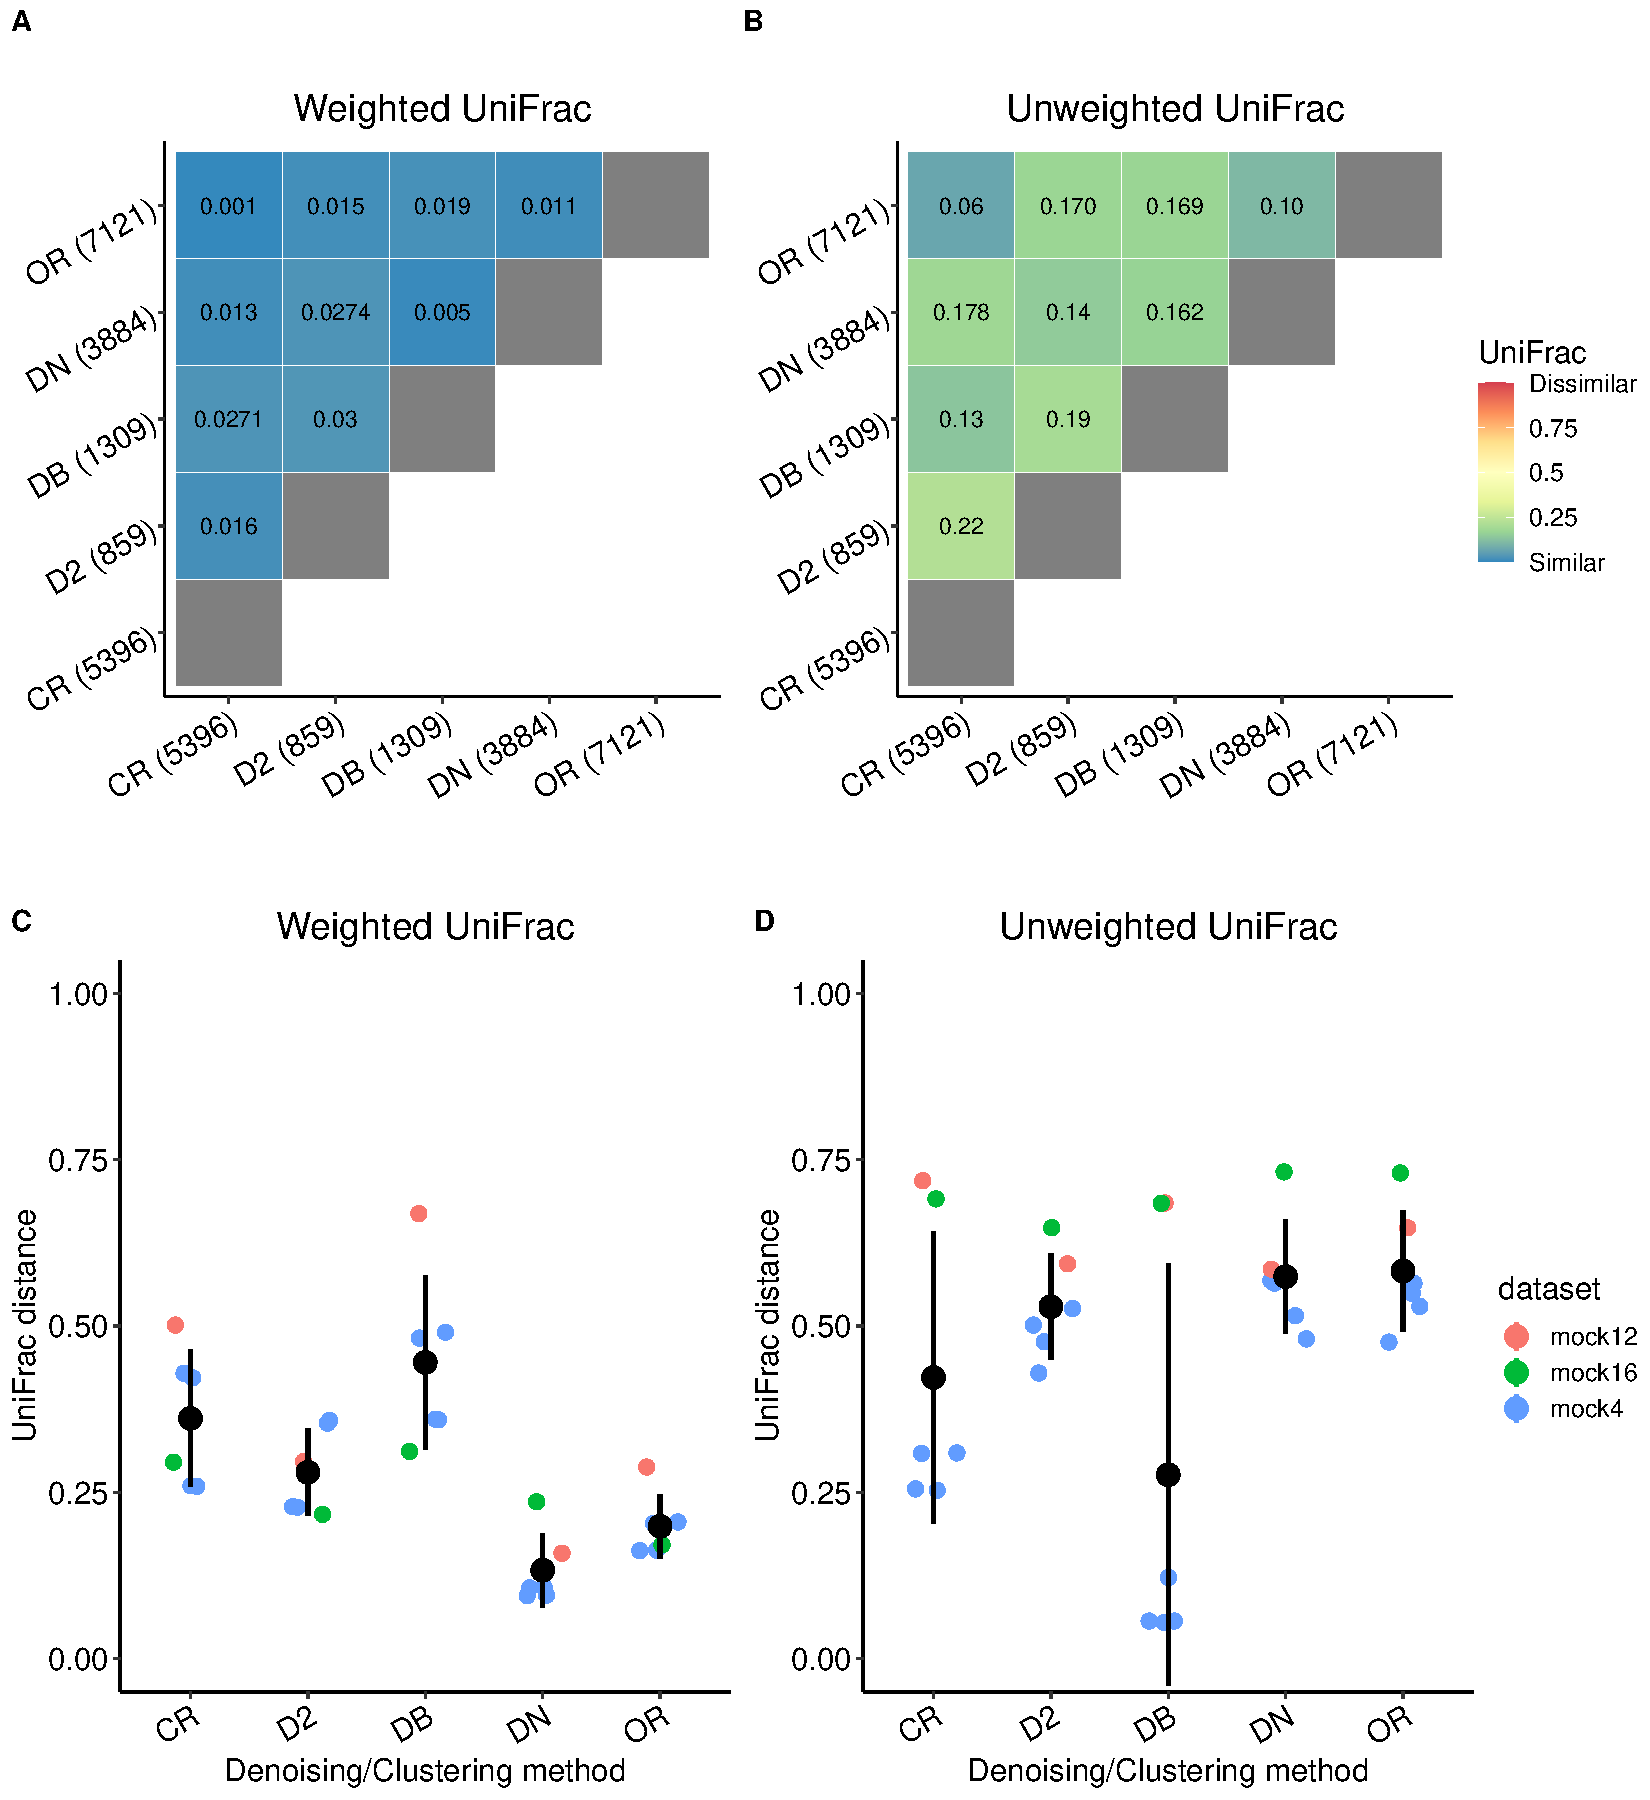
\includegraphics[width=1.0\linewidth]{figure2.pdf}
  \end{figure}
  \begin{figure}
    \centering
      \caption{
      \textbf{The choice of reference database contributes to the most variance in the networks}.
      \textbf{(A)} The total relative variance in the networks contributed by the DC, CC (chimera checking), TA and OP steps of the pipeline (right) and the linear model used to calculate the relative variance (left), see the Methods section for details.
      The analyses was performed on the healthy stool samples in a fecal microbiome transplant dataset~\ref{Kang2017}.
      The taxonomy database contributes most to the variance between the networks (65.4\%) followed by filtering of the counts matrix (26.8\%) in the OP step.
      \textbf{(B)} All combinations of inferred networks are shown as points on a PCA plot.
      Each point on the PCA plot represents a network inferred using different combinations of tools and parameters that are available in the \ac{micone} pipeline.
      The color of the points corresponds to the reference taxonomy database used to reconstruct those networks (left), and the network inference algorithm used to infer the networks (right).
      % TODO: The points aren't really separated
      The points on the PCA plot can be separated based on the TA step and the differences due to the DC and CC steps are comparatively not as significant.
    }
    \label{fig:figure2}
  \end{figure}
  \FloatBarrier
  \newpage

  \begin{figure}
    \centering
    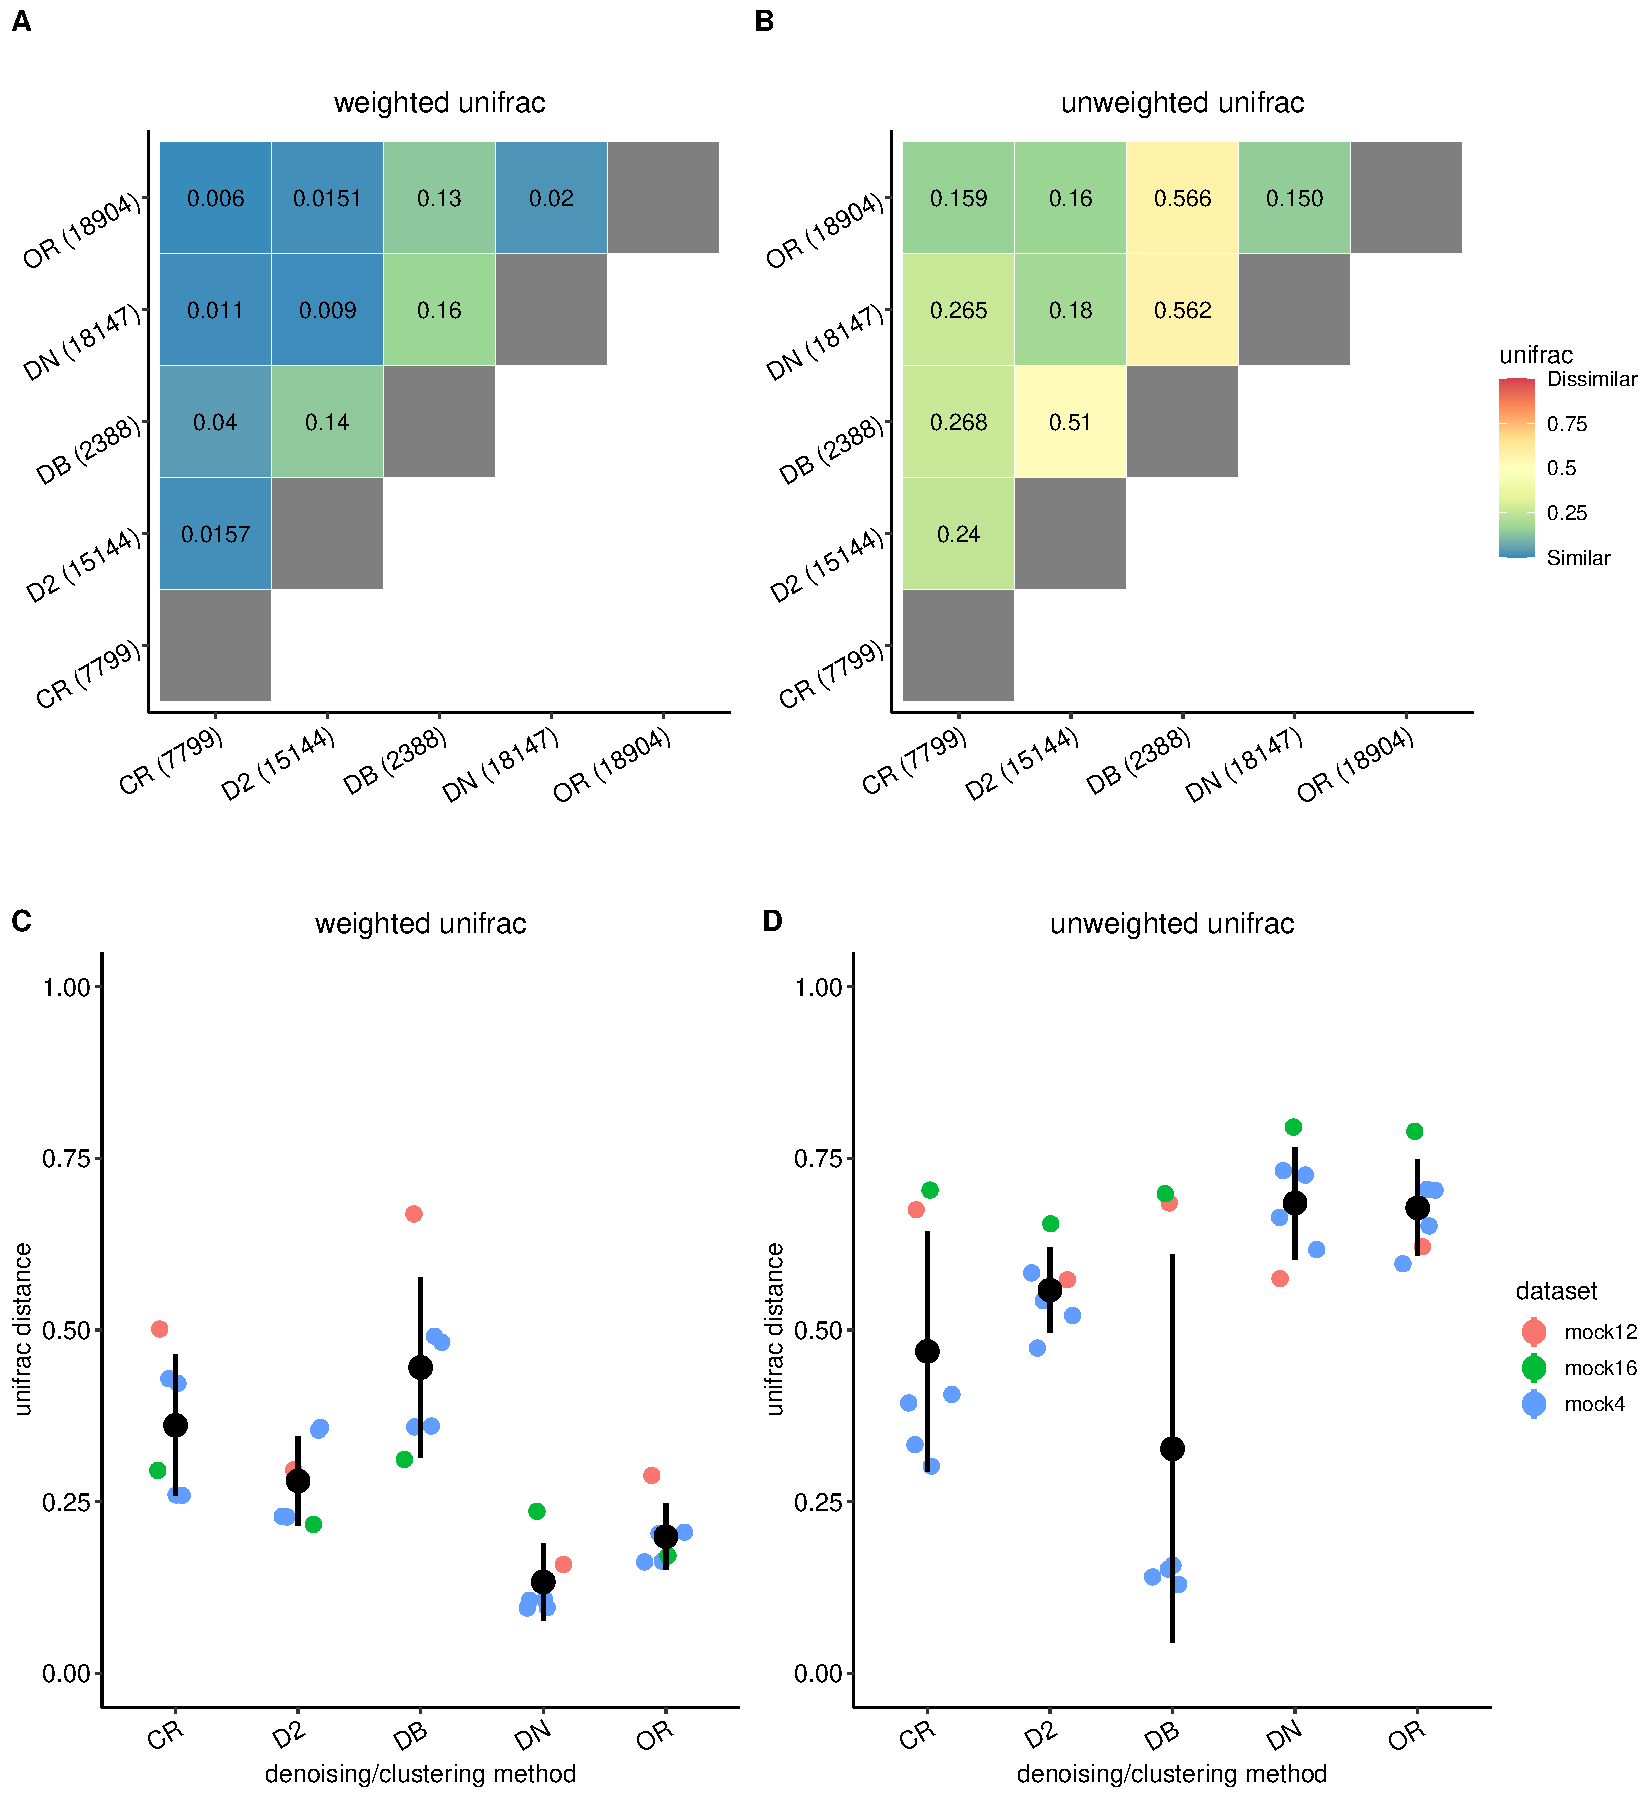
\includegraphics[width=\textwidth]{figure3.pdf}
  \end{figure}
  \begin{figure}
    \centering
    \caption{
      \textbf{The representative sequences generated by the different denoising/clustering methods are very similar but differ in the sequences that are lower in abundance.}
      \textbf{(A)} The average weighted UniFrac distance between the representative sequences shows that the representative sequences and their compositions are fairly identical between the methods (with the exception of Deblur (DB)).
      \textbf{(B)} The relatively larger average unweighted UniFrac distance indicates that methods differ in their identification of sequences that are lower in abundance.
      The number of \ac{otu}s or \ac{esv}s generated by the respective methods are provided in the parenthesis next to the names.
      \textbf{(C, D)} The distributions of the average weighted and unweighted UniFrac distance between the expected sequence profile and the calculated sequence profile in the mock datasets.
      The distributions of the average weighted UniFrac distance show that de novo (DN) and open reference (OR) were the best performing methods in most of the datasets, while they are worst performing methods under the unweighted UniFrac metric.
      The above average performance of dada2 (D2) under both distance metrics combined with its approach of identifying \ac{esv}s using de novo methods, prompts us to propose it as the default method for the DC step.
    }
    \label{fig:figure3}
  \end{figure}
  \FloatBarrier
  \newpage

  \begin{figure}[H]
    \centering
    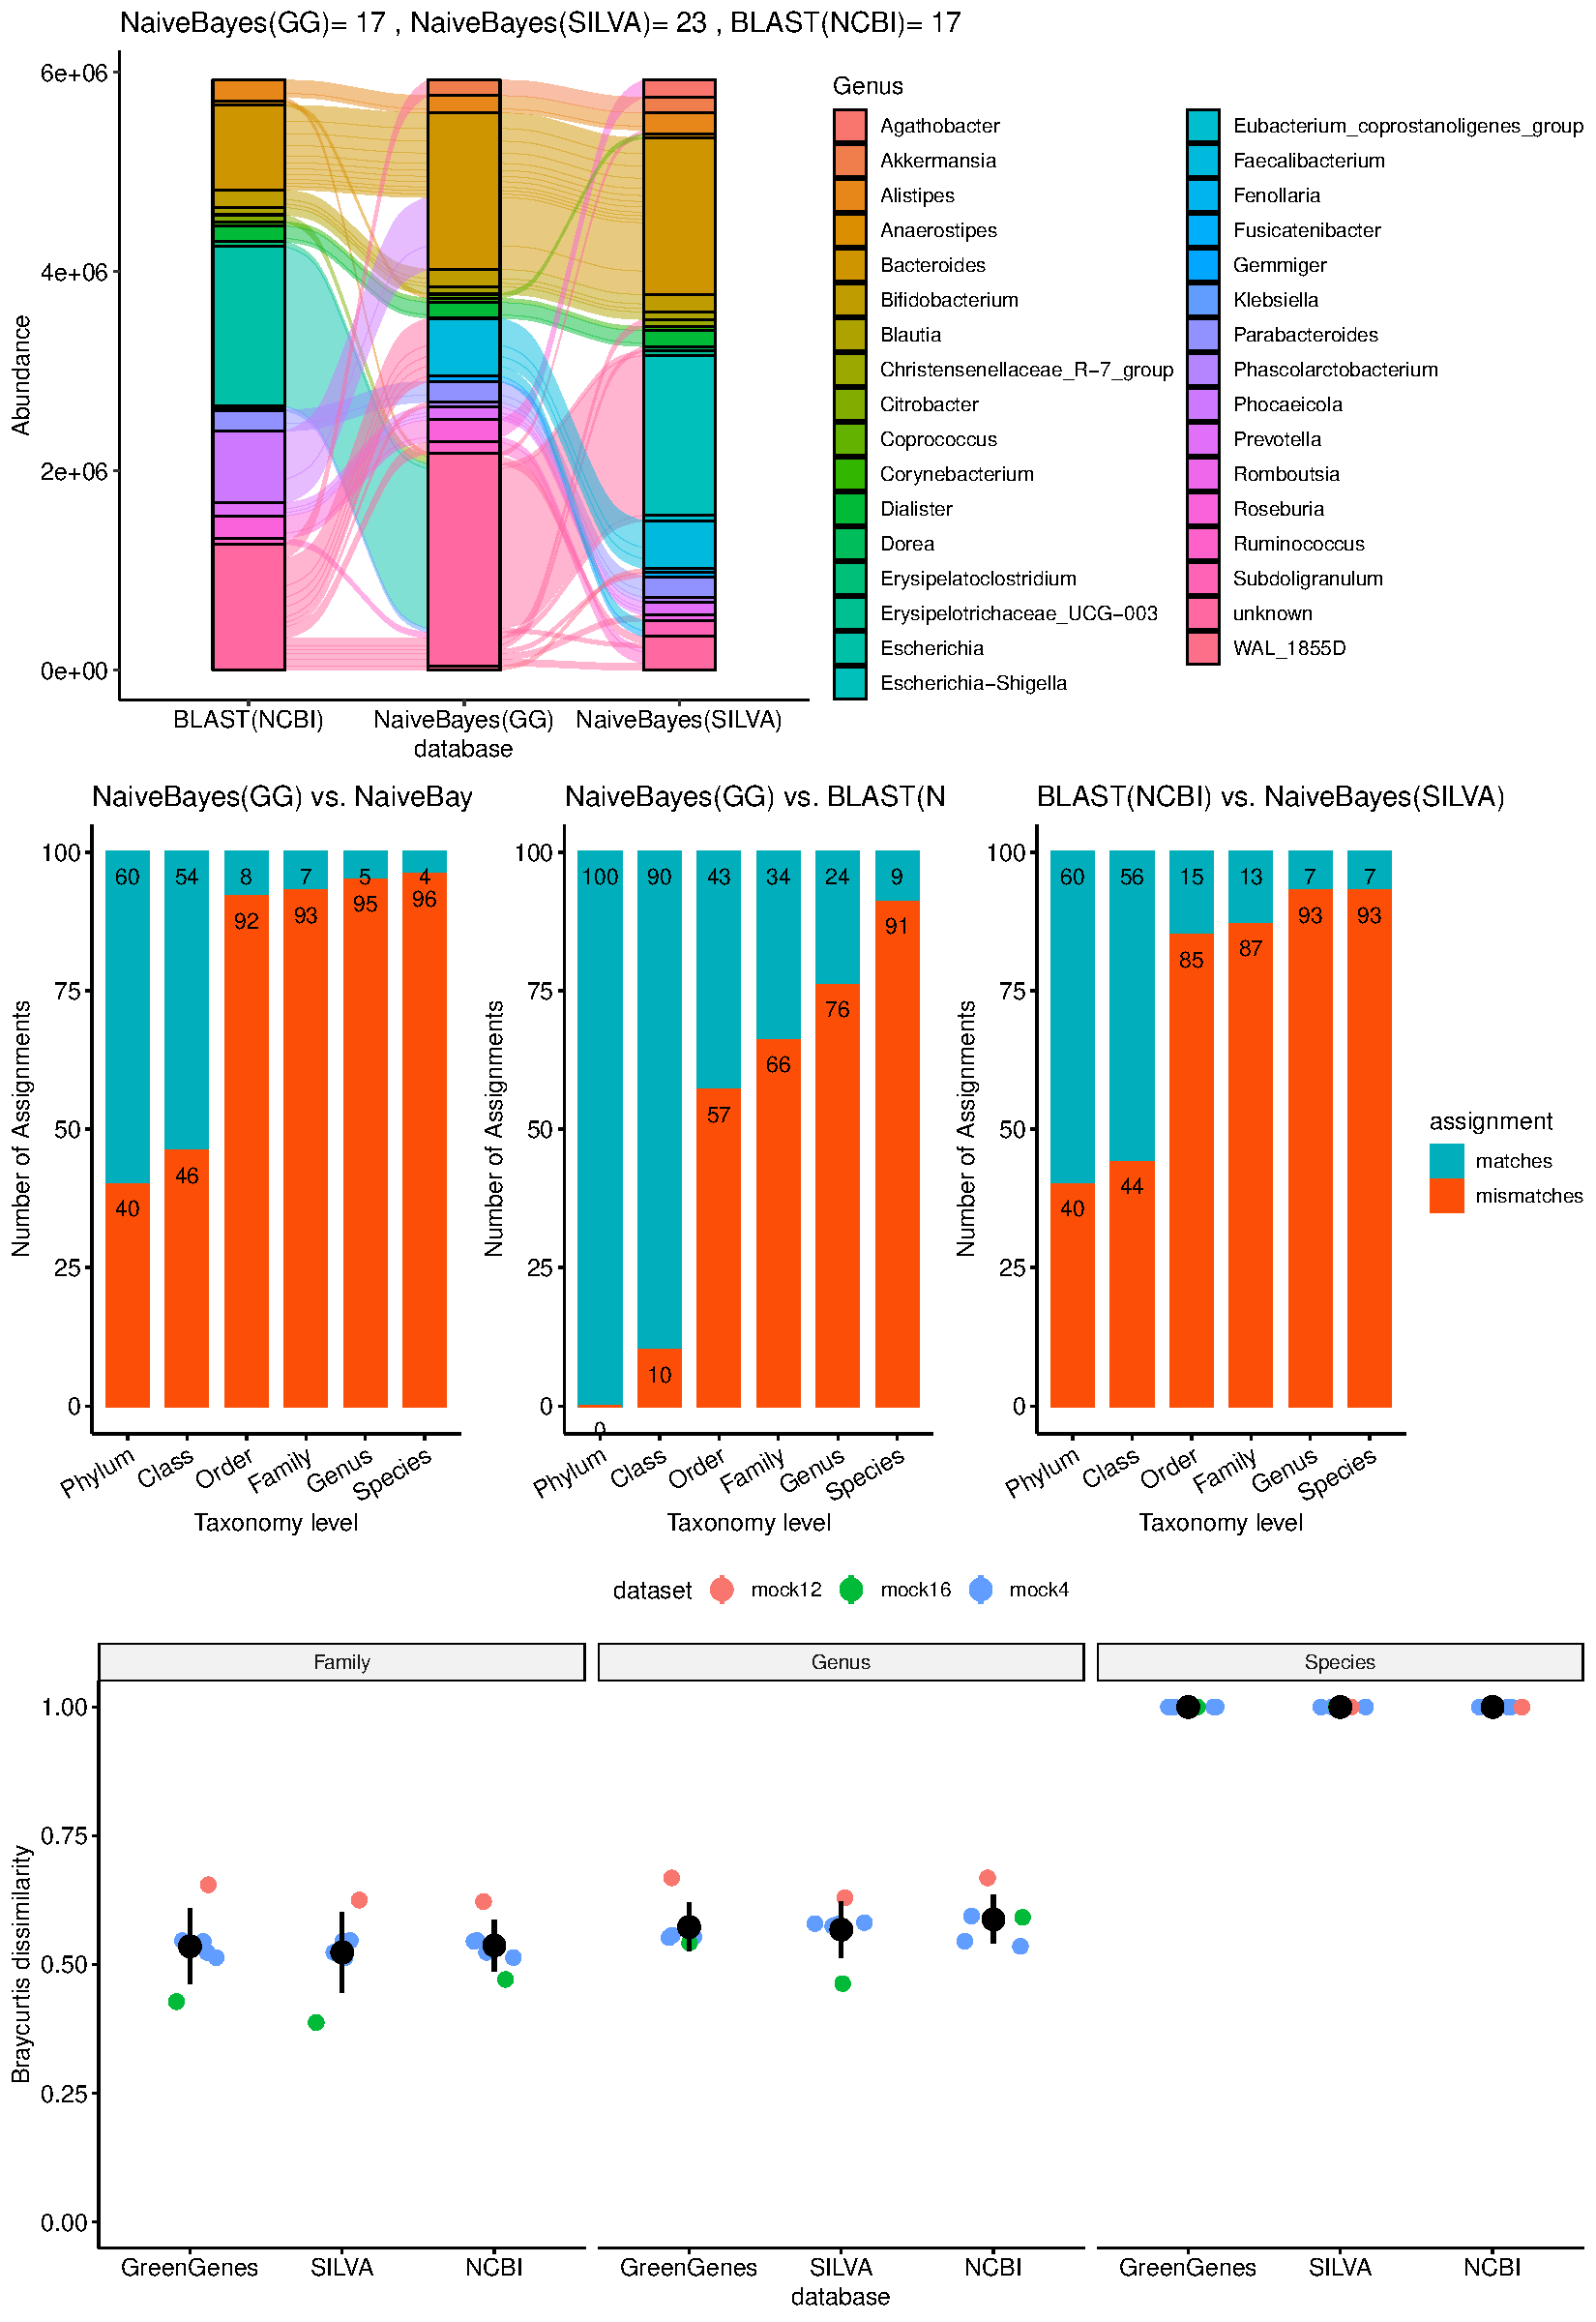
\includegraphics[width=\textwidth,height=1.2\textwidth]{figure4.pdf}
  \end{figure}
  \begin{figure}[H]
    \centering
    \caption{
      \textbf{Taxonomic reference databases vary widely in terms of their taxonomy assignments beyond the Order level.}
      \textbf{(A)} The assignments of the top 50 representative sequences to their respective taxonomies using the three different reference databases show how the same sequences are assigned to different Genus under the different databases.
      A significant portion of the representative sequences are assigned to an ``unknown'' Genus in two of three databases (\ac{gg} and \ac{ncbi}).
      \textbf{(B)} The number of representative sequences assigned to the same taxonomic label when using different reference databases, shown for the top 100 sequences.
      The number of mismatches are fewer at higher taxonomic levels but even at the Order level there exists greater than 51\% of mismatches, demonstrating the poor agreement in taxonomic labels assigned by the different databases.
      \textbf{(C)} The Bray-Curtis dissimilarity between the expected taxonomy profile and calculated taxonomy profile in the mock datasets shows that there is no singular best choice of database for every dataset, as all the databases have similar performance.
      However, we recommend the \ac{gg} database due to its popularity and if the goal is to compare against existing networks in literature.
    }
    \label{fig:figure4}
  \end{figure}
  \FloatBarrier
  \newpage


  \begin{figure}[H]
    \centering
    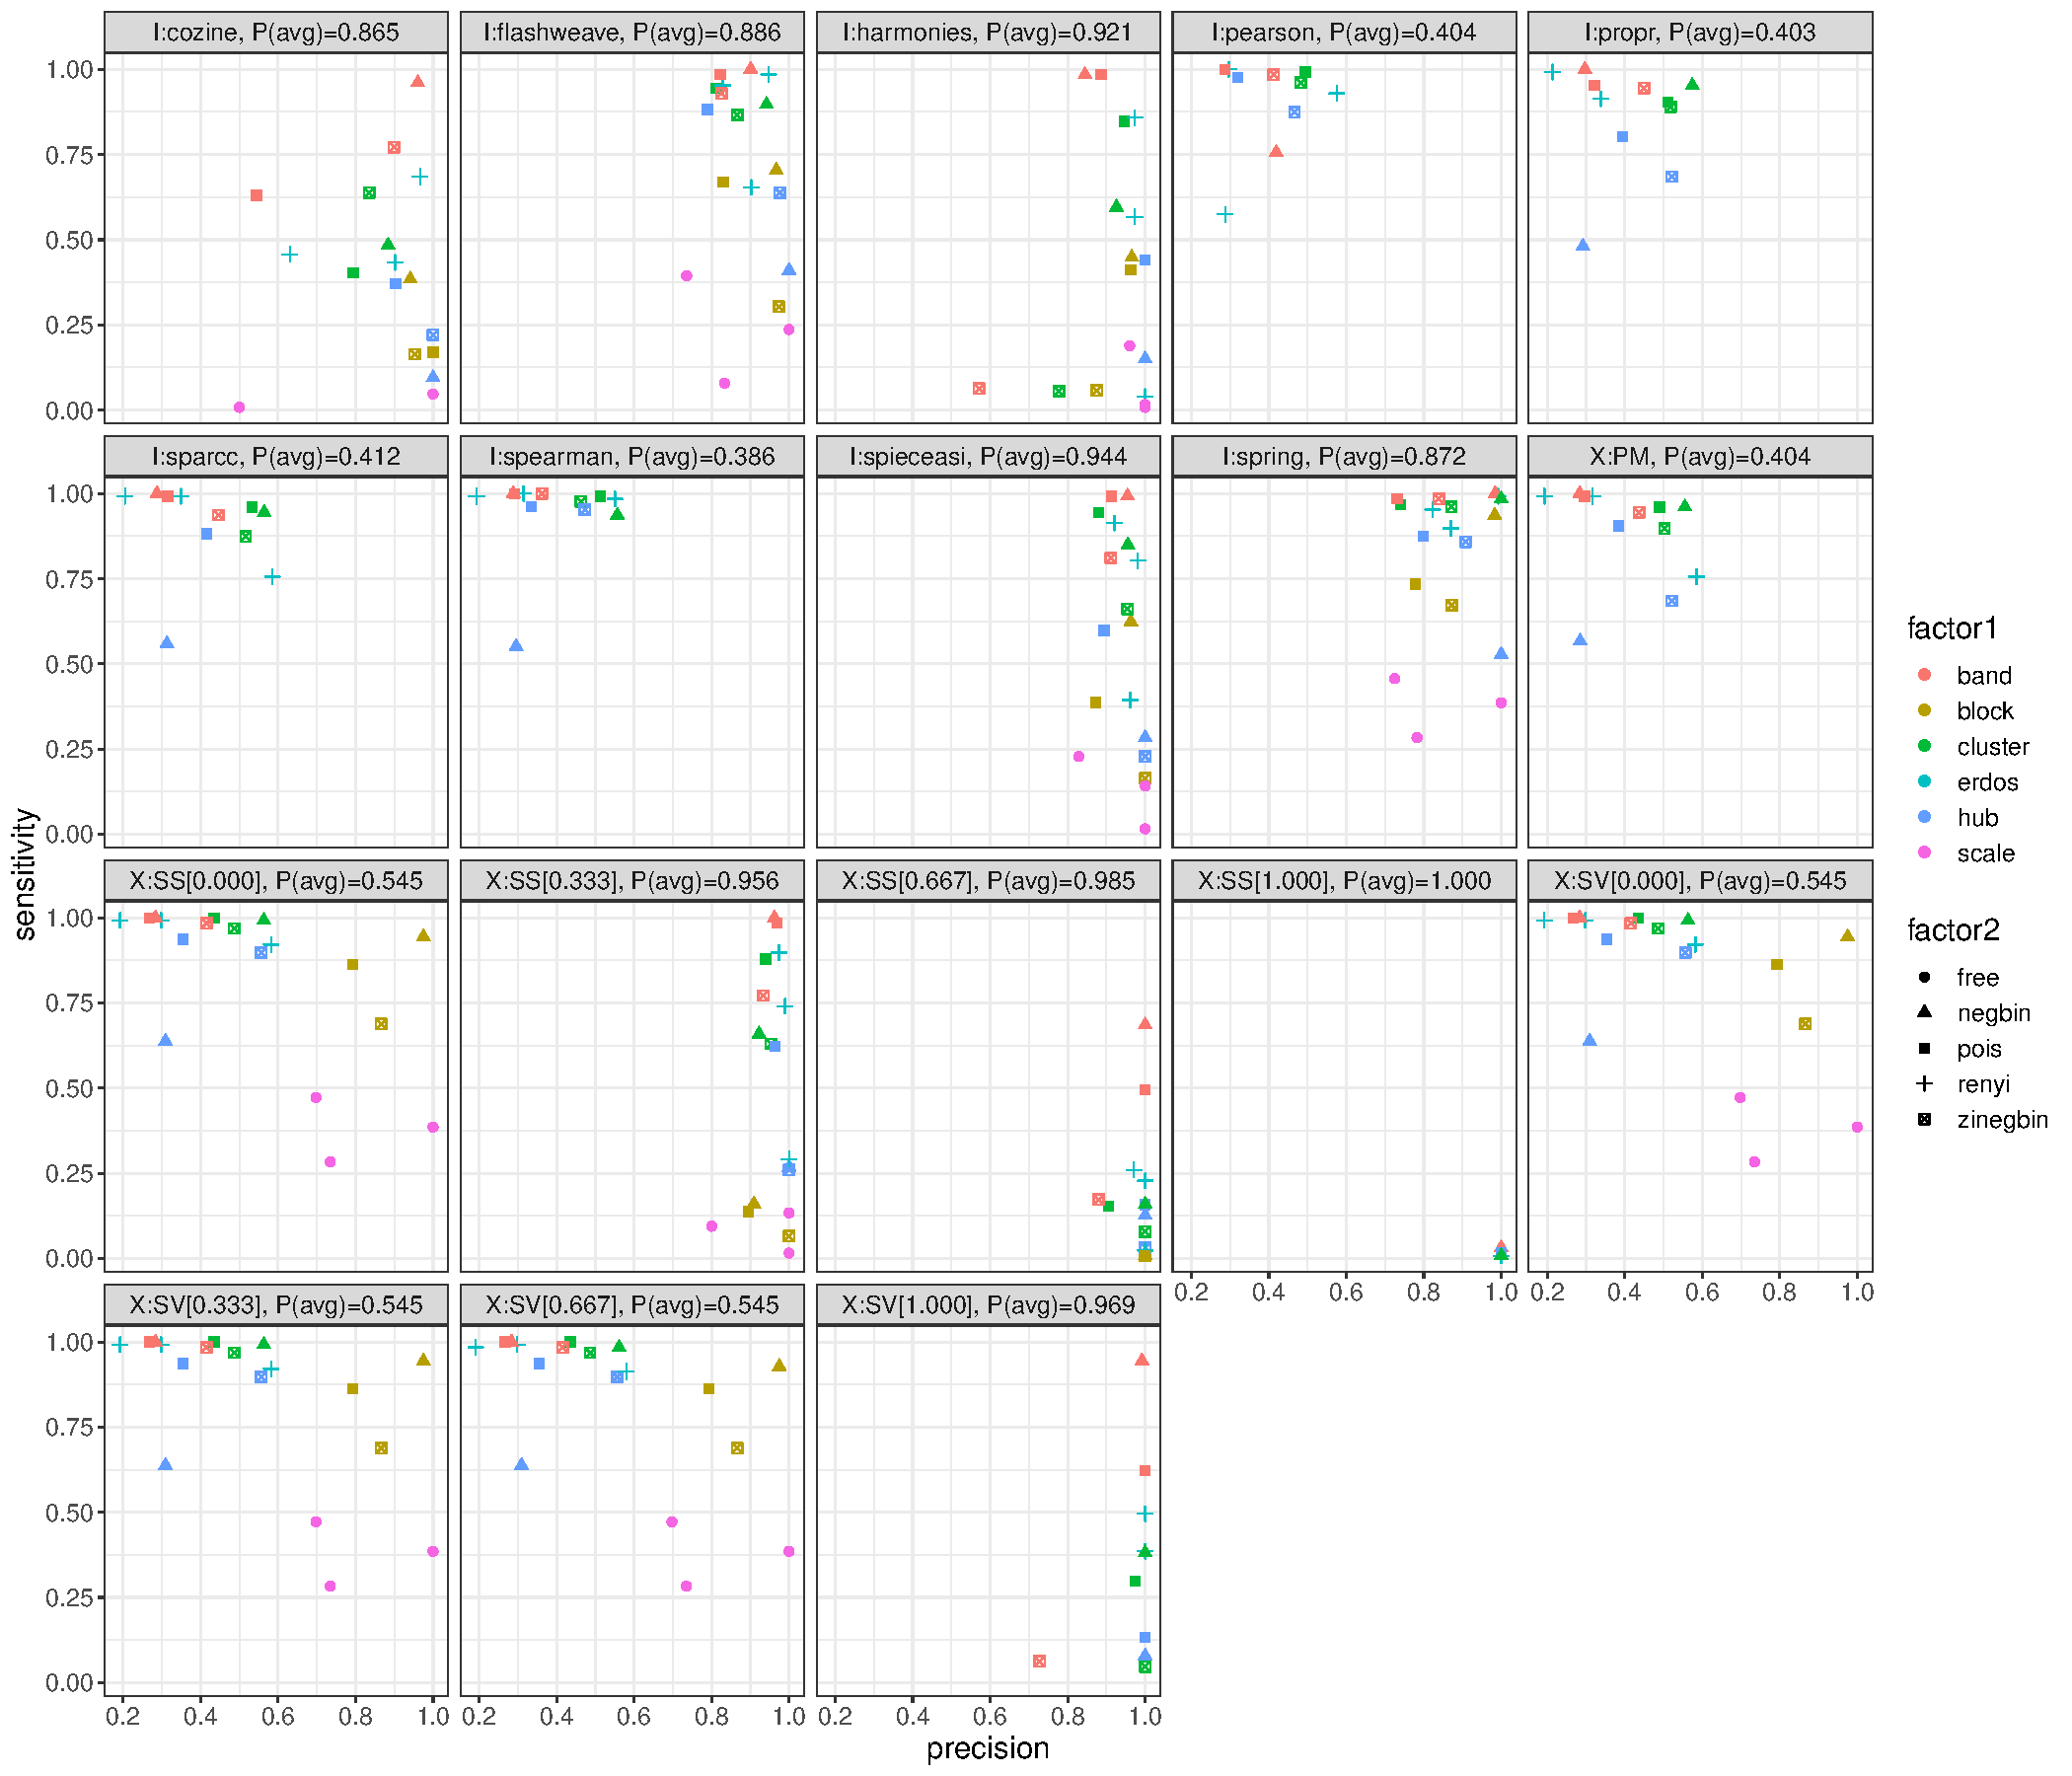
\includegraphics[width=\textwidth]{figure5.pdf}
  \end{figure}
  \begin{figure}[H]
    \centering
    \caption{
      \textbf{Networks generated using different network inference methods show notable differences both in terms of edge-density and connectivity}.
      \textbf{(A)} The nine different networks generated by the different network inference methods (excluding \ac{mldm}) are very dissimilar.
      The green links are positive associations and the orange links are negative associations.
      A threshold of 0.3 was set for the correlation-based methods (\ac{sparcc}, Propr, Spearman and Pearson) and a threshold of 0.01 was set for the other direct association methods.
      \textbf{(B)} The node overlap Upset plot indicates that all the networks have a large number of common nodes involved in connections (33 out of 68).
      Whereas, \textbf{(C)} the edge overlap Upset plot shows that a very small fraction of these connections are actually shared (8 out of 202).
    }
    \label{fig:figure5}
  \end{figure}
  \FloatBarrier
  \newpage

  \begin{figure}[h]
    \centering
    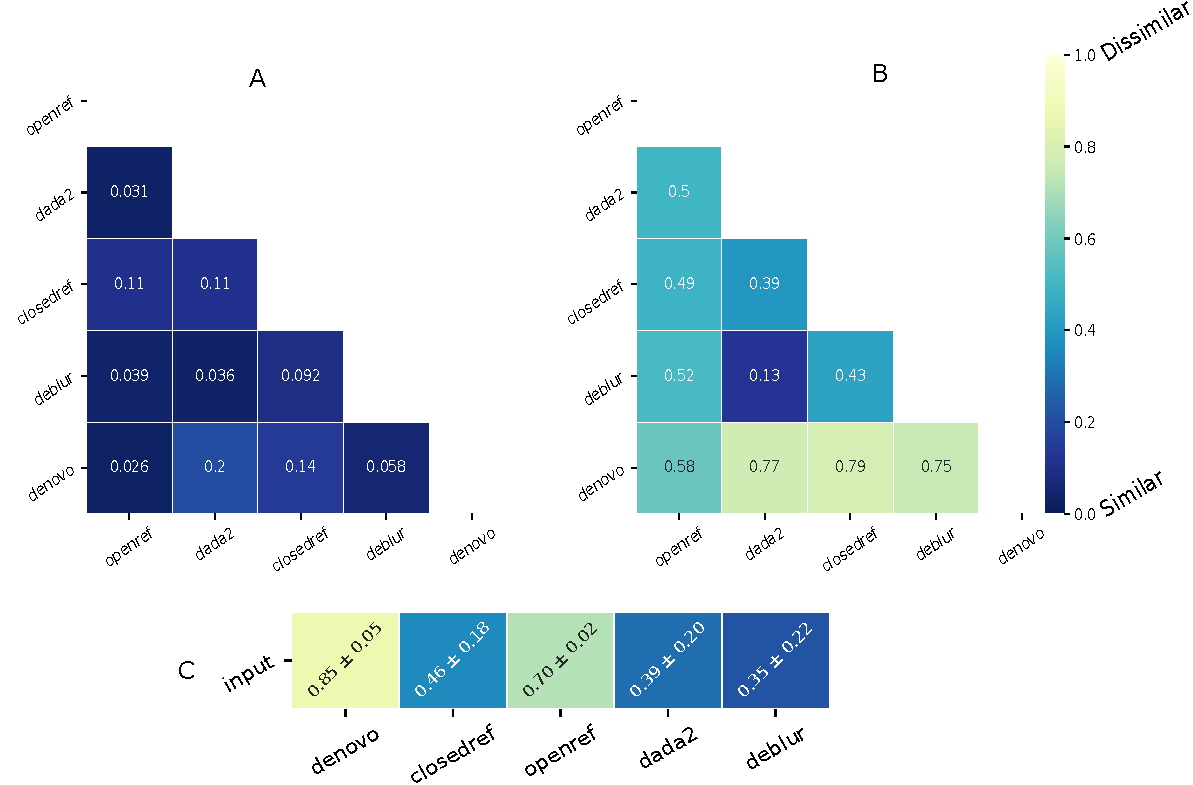
\includegraphics[width=1.0\linewidth]{figure6.pdf}
    \caption{
      \textbf{The precision and sensitivity of the inferred networks on the NorTA synthetic interaction data.}
      The ``I'' prefix indicates the individual network inference methods and the ``X'' prefix denotes the different consensus based methods.
      The different consensus based methods used are: pvalue merging (PM), scaled-sum (SS) and simple voting (SV) method.
      Pearson and Spearman methods are not used in the calculation of the consensus.
      Among all the independent network inference methods, \ac{spieceasi} has the best average precision (0.944), but the overall best precision was consistently obtained by the scaled-sum method (0.956, 0.985 and 1.000).
      The simple voting method when using presence of edges in all inferred networks as a requirement (parameter value 1.000), also outperforms \ac{spieceasi} on average precision (0.969).
      Therefore, we recommend the scaled-sum consensus method as the default tool for network inference.
    }
    \label{fig:figure6}
  \end{figure}
  \FloatBarrier
  \newpage

  % TODO: Verify the validity of Figure 7A and 7B again
  % Are they both using consensus?
  \begin{figure}[H]
    \centering
    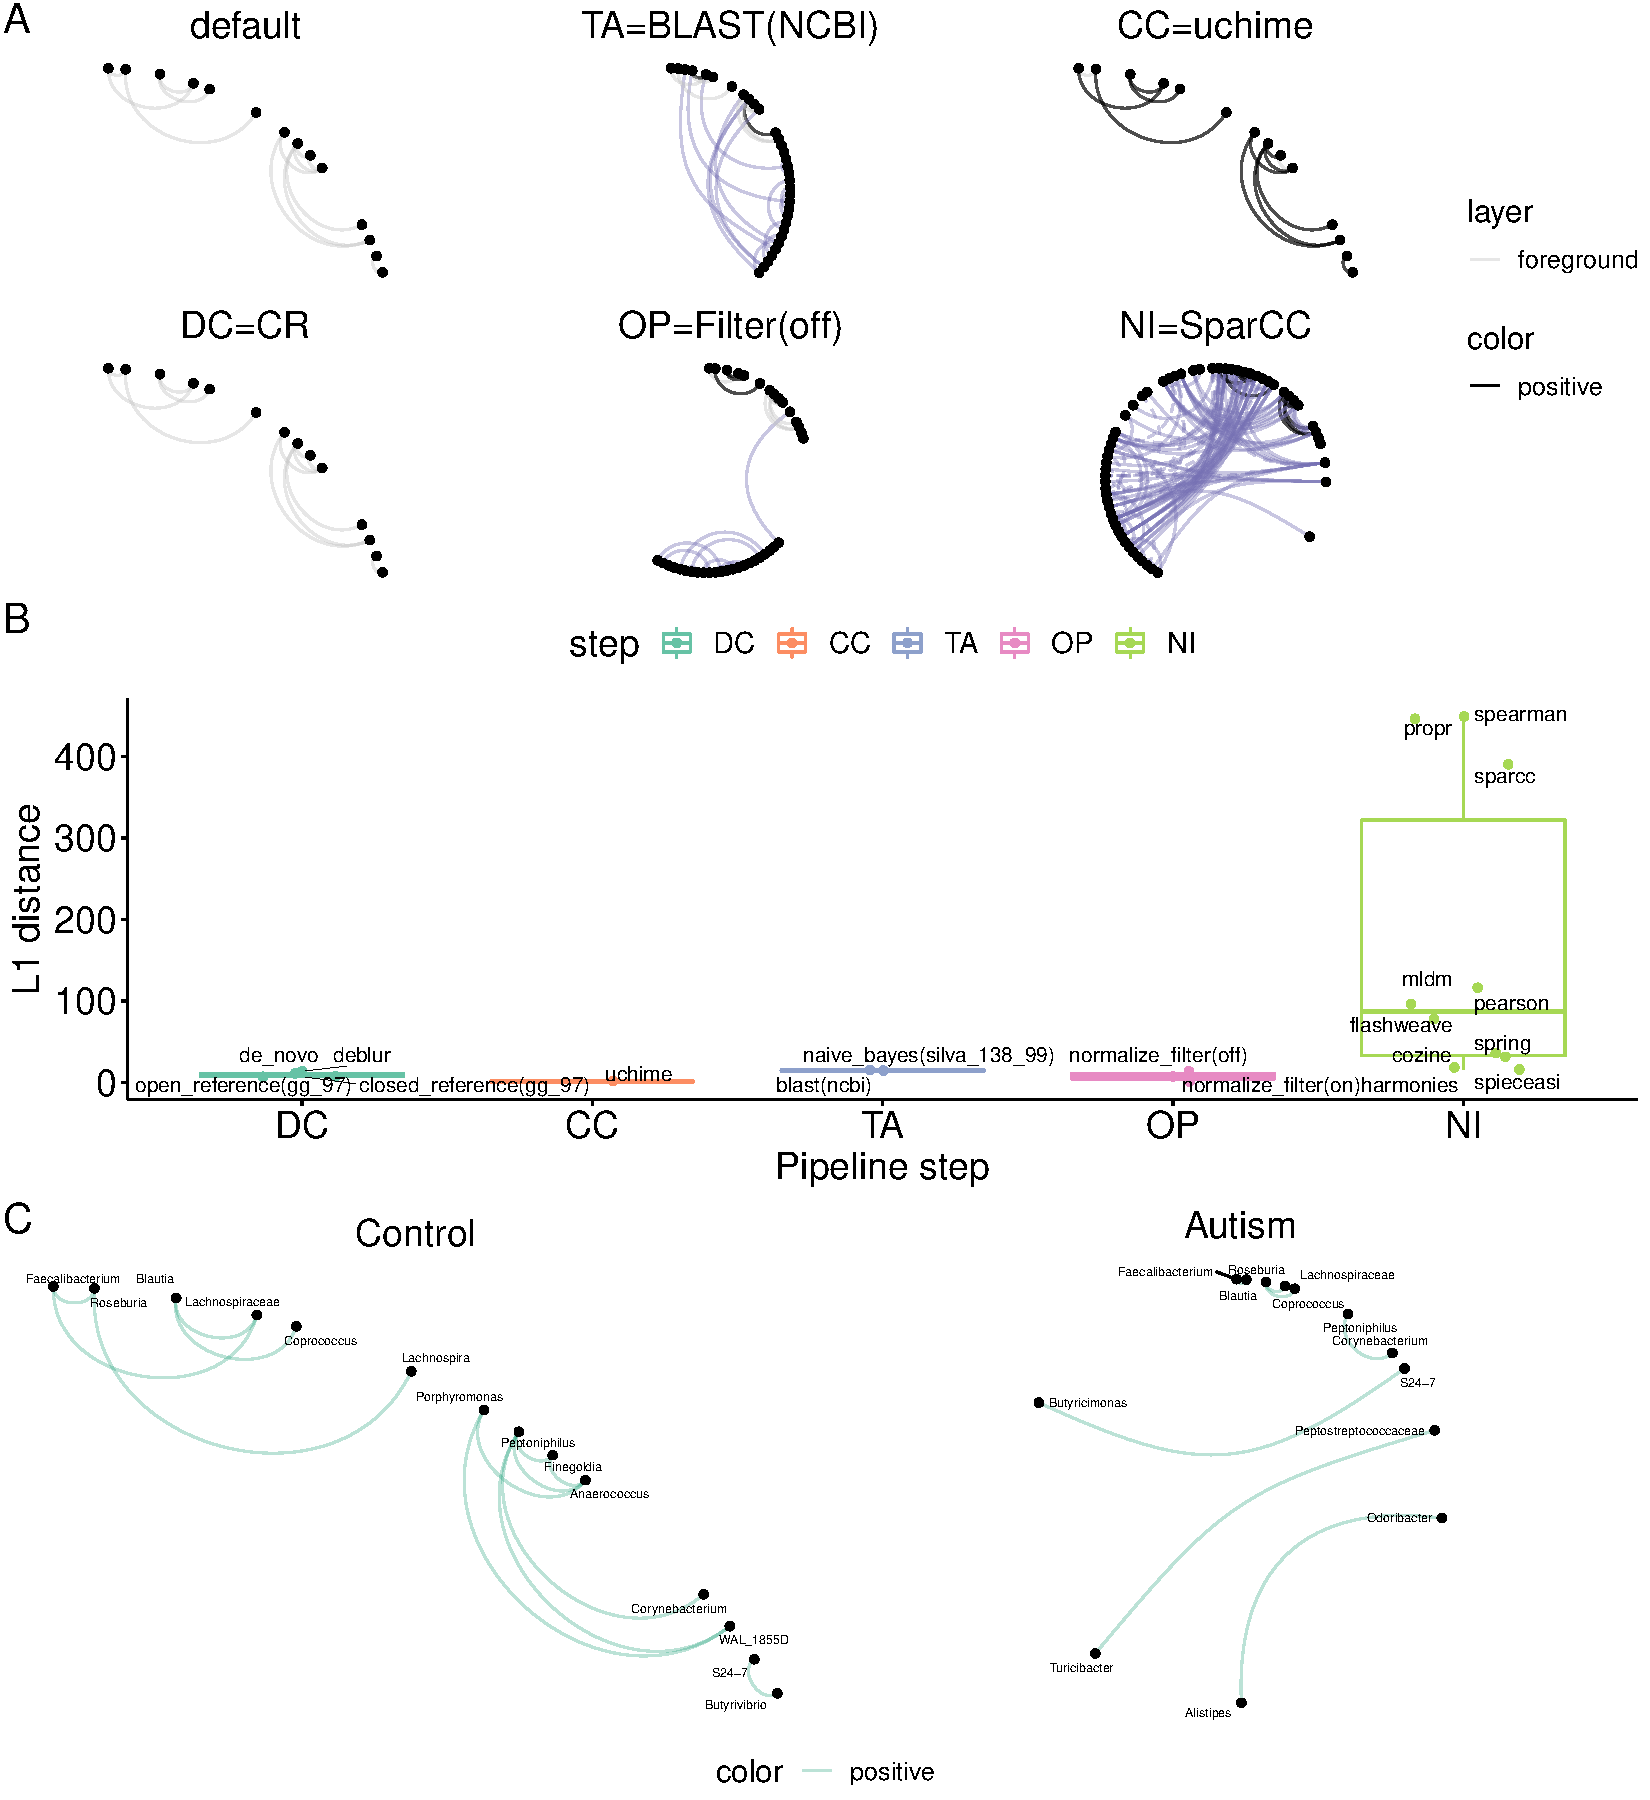
\includegraphics[width=1.0\linewidth]{figure7.pdf}
  \end{figure}
  \begin{figure}[H]
    \centering
    \caption{
      \textbf{The consensus algorithm drastically reduces variability in the networks and increases robustness of inferred networks}
      \textbf{(A)} The network constructed using the default pipeline parameters (DC=\ac{dada2}, CC=remove bimera, TA=\ac{gg}, OP=Filter(on), NI=scaled-sum consensus) is compared with networks generated when one of the steps use a different tool.
      The common connections (common with the default network) are in black, connections unique to the network are colored purple and connections in the default network but not present in the current network are gray.
      Changing the NI, TA and OP steps leads to the creation of the most number of new nodes and edges.
      \textbf{(B)} The boxplot showing the L1 distance between the networks generated by changing one step of the default pipeline and the network generated using the default parameters.
      The high value of L1 distances for the network inference step as compared to the other steps demonstrates how the consensus method is able to reduce the variability in the networks in the other steps of the pipeline.
      \textbf{(C)} The networks generated for the control (left) and autistic (right) samples in the fecal microbiome transplant dataset.
      These networks were generated using the default tools and parameters recommended by the \ac{micone} pipeline.
    }
    \label{fig:figure7}
  \end{figure}
